\chapter{Release 2: sprint 4 et sprint 5}

\section{Introduction}
La deuxième release enrichit la plateforme e-Gouvernement par des fonctionnalités de communication, de supervision et d'assistance. Elle se compose de deux sprints. Le \textit{Sprint 4} met en place la gestion des réclamations, le moteur de notifications automatisées et les outils de supervision de la plateforme. Le \textit{Sprint 5} livre le portail public, avec la vitrine institutionnelle et un assistant conversationnel intelligent fondé sur l'intelligence artificielle générative et une approche RAG, doublé d'un canal d'assistance permettant de recontacter les citoyens en difficulté.


\section{Sprint 4 : Réclamations, notifications et supervision}

Ce sprint permet aux citoyens de soumettre et suivre leurs réclamations, tout en offrant aux administrations des mécanismes de traitement structurés et un système de notifications assurant une communication fluide entre les acteurs. Il met également en place les outils de supervision : statistiques globales, journaux d'activités et logs système, qui donnent aux administrateurs une vue d'ensemble de l'activité de la plateforme et facilitent le diagnostic des anomalies.

\subsection{Backlog du Sprint 4}

Le tableau~\ref{tab:user-stories-sprint4}  présente le backlog du  sprint 4 avec l'estimation en jours de chaque tâche.

\renewcommand{\arraystretch}{1.3}

\begin{longtable}{|p{1cm}|p{3cm}|p{7cm}|p{1cm}|p{2cm}|}
\hline
\rowcolor{orange!30}
\textbf{ID} & \textbf{En tant que} & \textbf{User Story} & \textbf{Est/J} & \textbf{Priorité} \\
\hline
\endfirsthead

 

US22 & Administrateur Système & Je veux gérer les catégories de réclamations afin de mieux organiser et prioriser leur traitement & 2 & Élevée \\ \hline
US23 & Administrateur système & Je veux personnaliser les étapes de traitement des réclamations afin d'adapter le workflow au système & 2 & Élevée \\ \hline
US24 & Administrateur Institutionnel & Je veux gérer les réclamations soumises afin d'y apporter des réponses appropriées & 2 & Élevée \\ \hline
US25 & Administrateur Système & Je veux gérer les modèles de notifications afin de standardiser les messages envoyés aux utilisateurs & 2 & Élevée \\ \hline
US26 & Administrateur Système & Je veux gérer notifications afin d'informer automatiquement les utilisateurs des changements de statut & 2 & Élevée \\ \hline
US27 & Administrateur Système & Je veux consulter l'historique des notifications afin de suivre les communications envoyées & 2 & Moyenne \\ \hline
US28 & Internaute & Je veux gérer mes réclamations afin de signaler un problème rencontré sur la plateforme et de suivre leur statut de traitement & 2 & Élevée \\ \hline
US29 & Client & Je veux consulter mes notifications afin de rester informé des mises à jour concernant mes dossiers & 2 & Élevée \\ \hline
US30 & Administrateur & Je veux consulter les statistiques globales par administration afin d'analyser l'activité de la plateforme & 2 & Moyenne \\ \hline
US31 & Administrateur & Je veux consulter les journaux d'activités par administration afin de surveiller les actions effectuées & 1 & Moyenne \\ \hline
US32 & Administrateur Système & Je veux consulter les logs système afin de détecter les anomalies et assurer la sécurité & 1 & Moyenne \\ \hline

\rowcolor{white}
\caption{Backlog du Sprint 4}
\label{tab:user-stories-sprint4}
\end{longtable}

\subsection{Diagramme de cas d’utilisation du sprint 4}

La figure \ref{fig:cas-utilisation-sprint4},présente le diagramme de cas d'utilisation du sprint 4.

\begin{figure}[H]
    \centering
    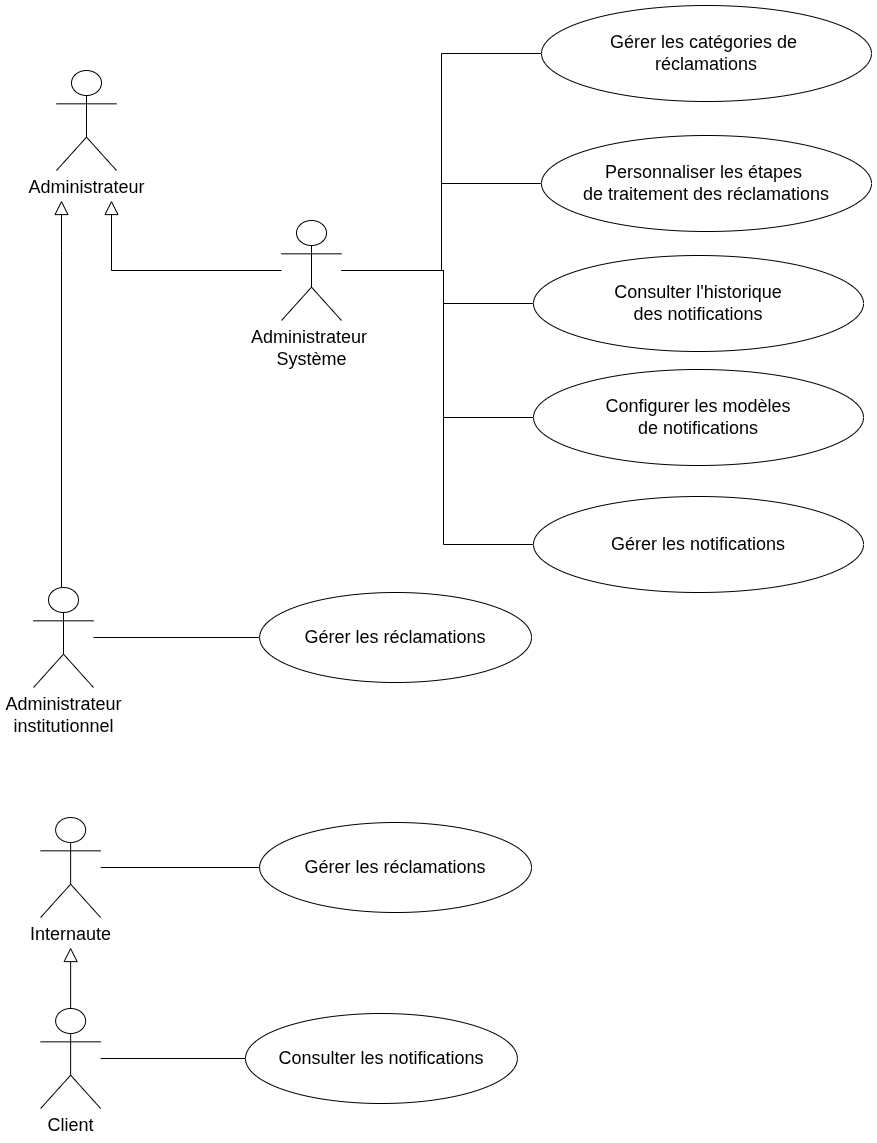
\includegraphics[width=10cm,height=20cm]{images/diagrammes/sprint4/cas-utilisation-sprint4.drawio.png}
    \caption{Diagramme de cas d'utilisation -- Sprint 4}
    \label{fig:cas-utilisation-sprint4}
\end{figure}

\subsection{Diagramme de classe du Sprint 4}
La figure \ref{fig:classe-sprint4}, présente le diagramme de classe du sprint 4.

\begin{figure}[H]
    \centering
    \includegraphics[width=18cm,height=16cm]{images/diagrammes/sprint4/diag-classe-sprint4.drawio.png}
    \caption{Diagramme de classe -- Sprint 4}
    \label{fig:classe-sprint4}
\end{figure}

\subsection{Raffinement et description textuelle du cas d'utilisation <<Personnaliser les étapes de traitement des réclamations >>}

Dans la section suivante, nous utiliserons des descriptions de
scénarios pour décrire le cas « Personnaliser les étapes
de traitement des réclamations ». Ce dernier montre les sous-opérations possibles à faire.


La figure \ref{fig:cas-utilisation-sprint4-raff}, présente le diagramme de cas d'utilisation raffiné du cas d'utilisation « Personnaliser les étapes
de traitement des réclamations ».
\begin{figure}[H]
    \centering
    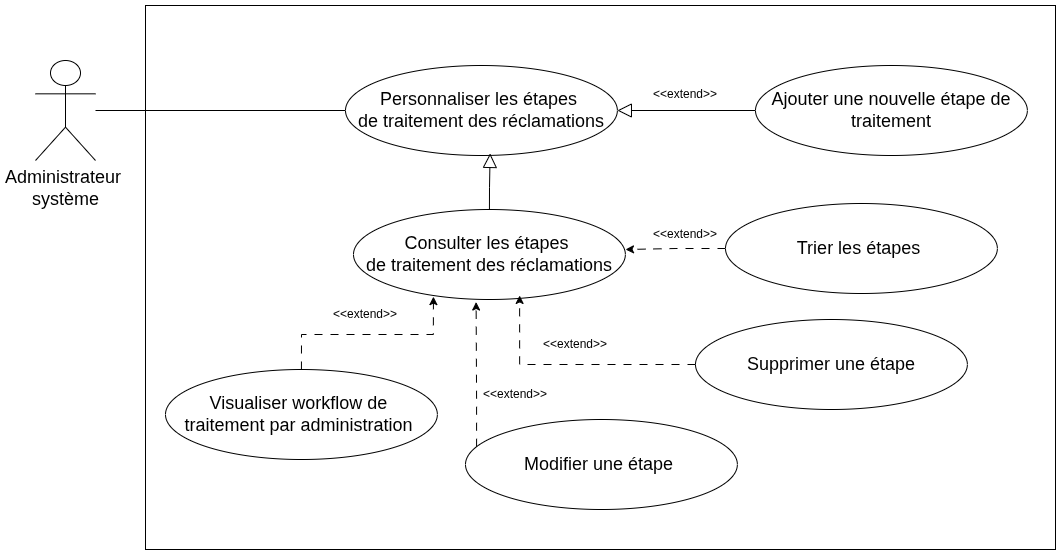
\includegraphics[width=15cm,height=10cm]{images/diagrammes/sprint4/cas-utilisation-personaliser-reclamation-raff.drawio_2.png}
    \caption{Raffinement du cas d'utilisation « Personnaliser les étapes
de traitement des réclamations »}
    \label{fig:cas-utilisation-sprint4-raff}
\end{figure}

\textbf{Description textuelle}

% ===================== AJOUTER =====================
Une description détaillée du cas d’utilisation « Ajouter une nouvelle étape de traitement » est présentée dans le tableau~\ref{tab:ajouter-etape-traitement}.

 \renewcommand{\arraystretch}{1.3}

\begin{longtable}{|p{4cm}|p{12cm}|}
\hline
\rowcolor{gray!20}
\textbf{Champ} & \textbf{Description} \\ 
\hline
\endfirsthead

 

Nom & Ajouter une nouvelle étape de traitement \\ \hline

Acteur principal & Administrateur système \\ \hline

Objectif & Permettre l’ajout d’une nouvelle étape dans le workflow de traitement des réclamations. \\ \hline

Pré-condition &
\begin{itemize}
    \item Une administration est sélectionnée.
\end{itemize}
\\ \hline

Scénario nominal &
\begin{enumerate}
    \item L’administrateur clique sur « Ajouter une étape ».
    \item Il renseigne les informations de l’étape (nom, ordre, administration, statut).
    \item Il valide les informations saisies.
    \item Le système enregistre la nouvelle étape.
\end{enumerate}
\\ \hline

Scénario alternatif &
\begin{itemize}
    \item Si les champs sont invalides, un message d’erreur est affiché.
\end{itemize}
\\ \hline

Post-condition &
La nouvelle étape est ajoutée au workflow. \\ \hline

\caption{Description textuelle : Ajouter une nouvelle étape de traitement}
\label{tab:ajouter-etape-traitement}

\end{longtable}


% ===================== VISUALISER =====================
Une description détaillée du cas d’utilisation « Visualiser workflow de traitement par administration » est présentée dans le tableau~\ref{tab:visualiser-workflow-traitement}.

\renewcommand{\arraystretch}{1.3}

\begin{longtable}{|p{4cm}|p{12cm}|}
\hline
\rowcolor{gray!20}
\textbf{Champ} & \textbf{Description} \\ 
\hline
\endfirsthead

\hline
\rowcolor{gray!20}
\textbf{Champ} & \textbf{Description} \\ 
\hline
\endhead

Nom & Visualiser workflow de traitement par administration \\ \hline

Acteur principal & Administrateur système \\ \hline

Objectif & Permettre la visualisation complète du workflow de traitement des réclamations d’une administration. \\ \hline

Pré-condition &
\begin{itemize}
    \item Une administration est sélectionnée.
\end{itemize}
\\ \hline

Scénario nominal &
\begin{enumerate}
    \item L’administrateur clique sur workflow de traitement.
    \item Le système affiche le workflow complet de chaque administration.
    \item Les étapes sont affichées dans leur ordre de traitement.
\end{enumerate}
\\ \hline

Scénario alternatif &
\begin{itemize}
    \item Aucun workflow n’est disponible : affichage d’un message informatif.
\end{itemize}
\\ \hline

Post-condition &
Le workflow est consulté avec succès. \\ \hline

\caption{Description textuelle : Visualiser workflow de traitement}
\label{tab:visualiser-workflow-traitement}

\end{longtable}


\subsection{Les diagrammes de séquences du cas d’utilisation « Personnaliser les étapes de traitement des réclamations »}

Dans cette section, nous avons choisi de présenter certains diagrammes de séquence parmi ceux définis lors de l’étape de raffinement du sprint « Gestion des étapes de traitement des réclamations ». Ce choix vise à mettre en évidence les interactions les plus représentatives du système, notamment la consultation du workflow, la visualisation des étapes, ainsi que les opérations d’ajout, de modification et de suppression d’une étape. Ces diagrammes permettent d’illustrer le fonctionnement global du processus de gestion des réclamations et les échanges entre l’administrateur et le système.

\noindent  \textbf{Présentation des diagrammes de séquences :}



% ===================== WORKFLOW =====================
Le diagramme de séquence de la figure~\ref{fig:workflow-etapes} décrit le processus de visualisation du workflow de traitement des réclamations par l'administration. Il permet à l’administrateur de visualiser toutes les étapes du processus de gestion des réclamations.

\begin{figure}[H]
    \centering
    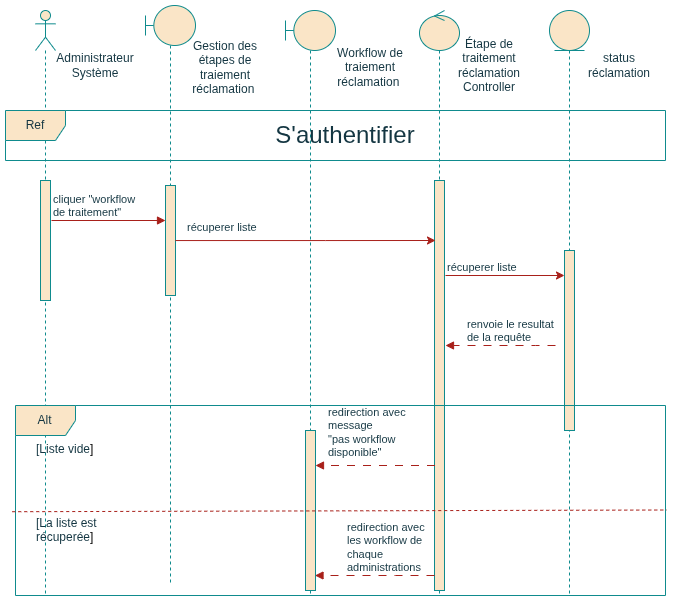
\includegraphics[width=15cm,height=16cm]{images/diagrammes/sprint4/workflow_etape.drawio.png}
    \caption{Diagramme de séquence - Visualiser workflow de traitement par administration}
    \label{fig:workflow-etapes}
\end{figure}


% ===================== AJOUTER =====================
La figure ~\ref{fig:ajouter-etape} décrit, sous forme de diagramme de séquence, le déroulement de l'ajout d'une nouvelle étape dans le traitement des réclamations. Elle met en évidence les échanges permettant à l'administrateur de créer puis d'enregistrer cette étape au sein du workflow déjà en place. 

\begin{figure}[H]
    \centering
    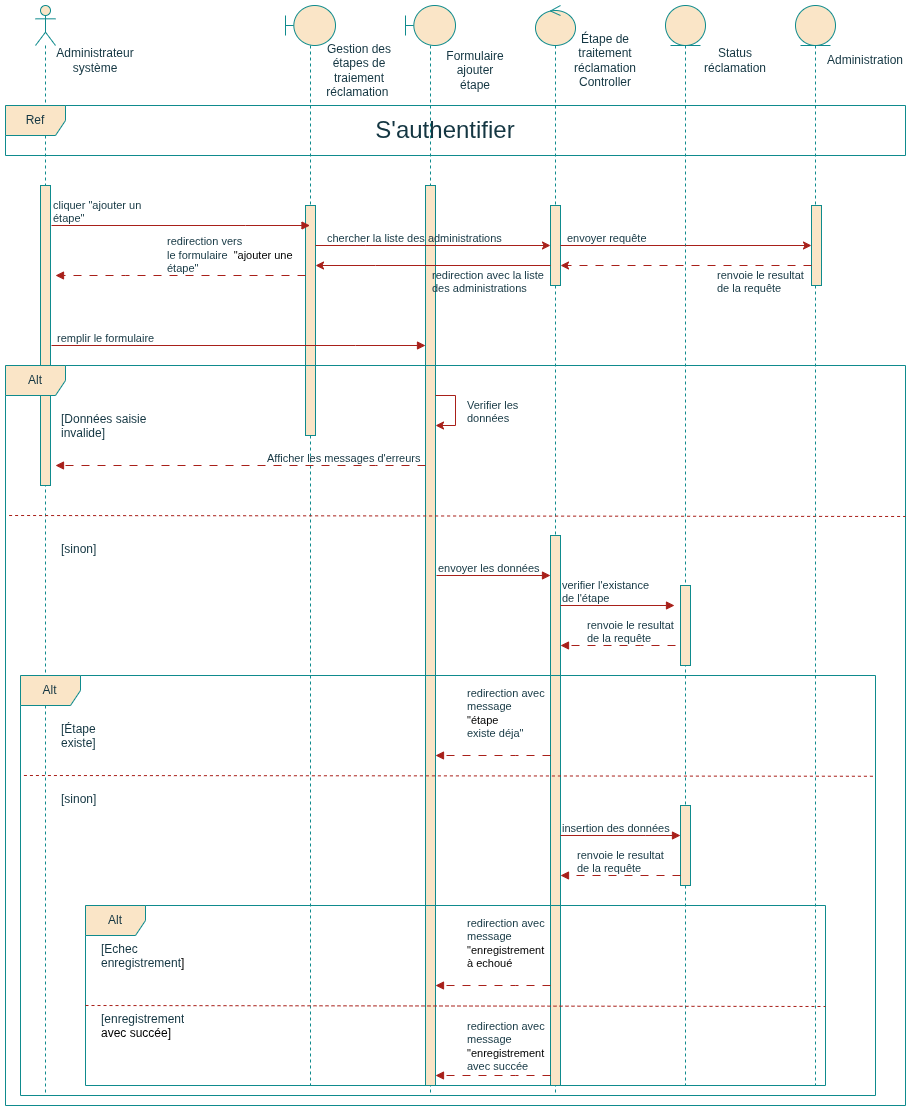
\includegraphics[width=15cm,height=16cm]{images/diagrammes/sprint4/ajouter-etape.drawio.png}
    \caption{Diagramme de séquence - Ajouter une nouvelle étape de traitement}
    \label{fig:ajouter-etape}
\end{figure}


\subsection{Réalisation du sprint <<Personnaliser les étapes de traitement des réclamations>>}

Dans cette section, nous présentons certaines interfaces représentatives de la réalisation du sprint « Gestion des étapes de traitement des réclamations », afin d’illustrer les principales fonctionnalités implémentées. Ce choix met en évidence les écrans les plus significatifs du système, notamment la consultation des étapes, la visualisation du workflow ainsi que les opérations de modification et de suppression. Ces captures permettent de mieux comprendre la structuration du processus de traitement des réclamations et l’interaction de l’administrateur avec le système.

\noindent \textbf{Présentation des interfaces :}

% ===================== CONSULTER =====================
La figure~\ref{fig:etapes-reclamations} présente l’interface de consultation des étapes de traitement des réclamations associées à plusieurs administration.


\begin{figure}[H]
    \centering
    \fbox{%
        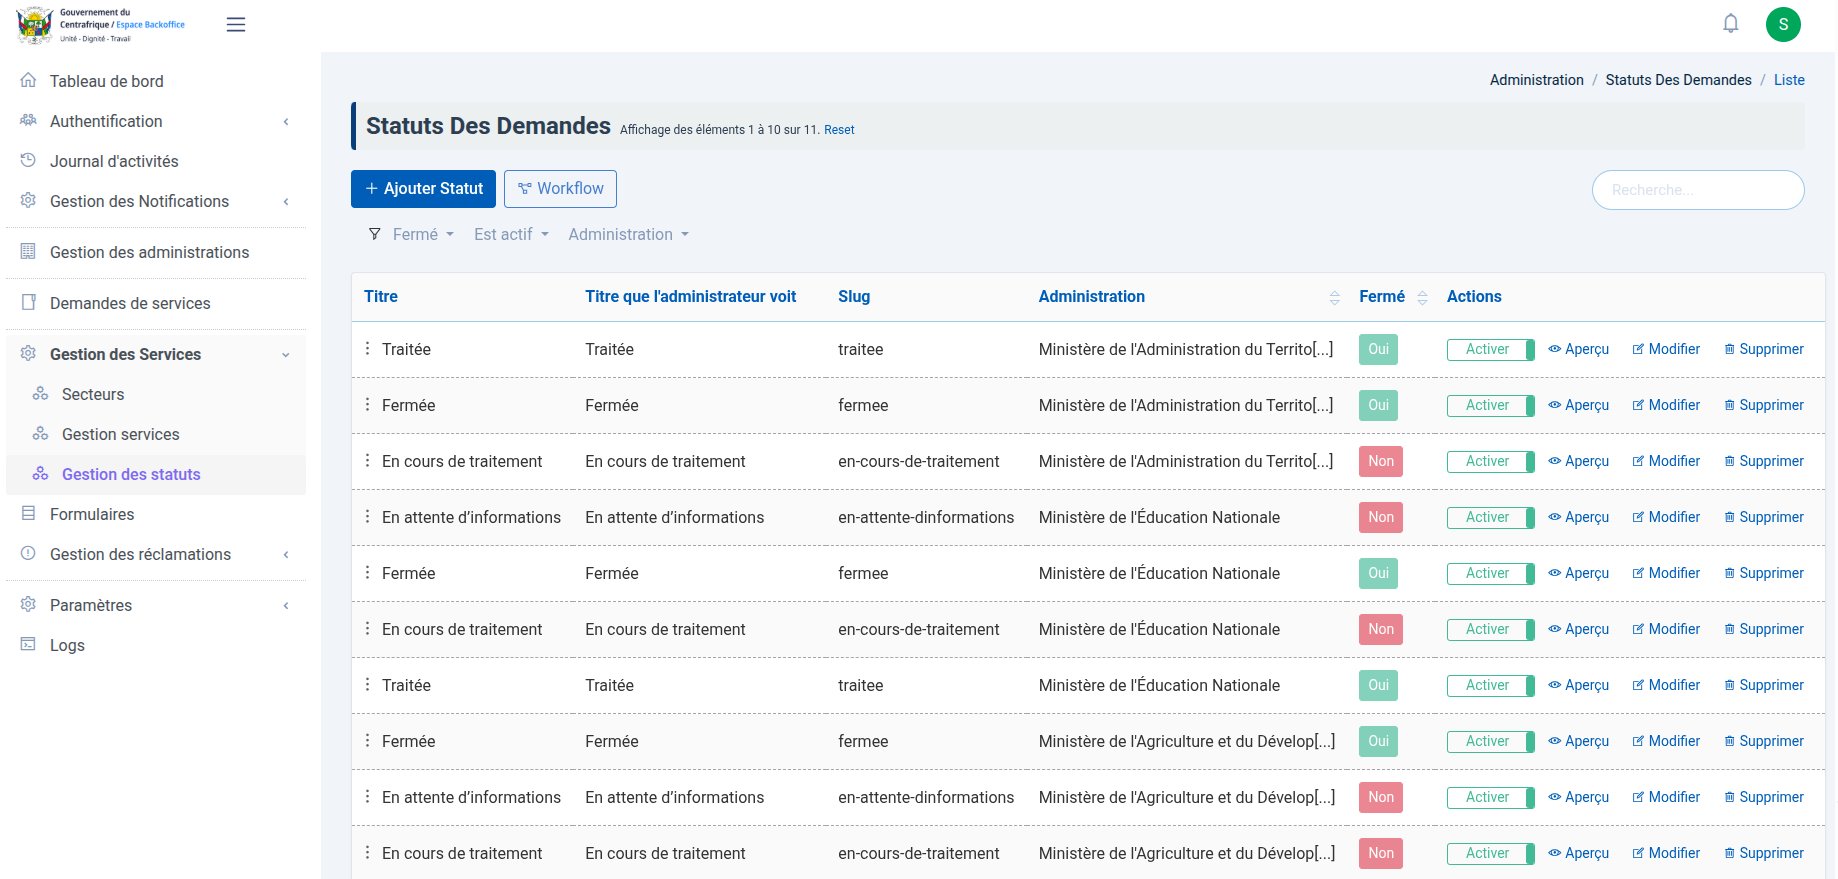
\includegraphics[width=0.95\textwidth]{images/realisation/sprint4/list.png}
    }
    \caption{Consultation des étapes de traitement des réclamations}
    \label{fig:etapes-reclamations}
\end{figure}






% ===================== WORKFLOW =====================

La figure~\ref{fig:workflow-traitement} présente l’interface qui permet de visualiser le workflow complet de traitement des réclamations par administration. Elle met en évidence l’enchaînement des étapes et leur organisation dans le processus global.

\begin{figure}[H]
    \centering
    \fbox{%
        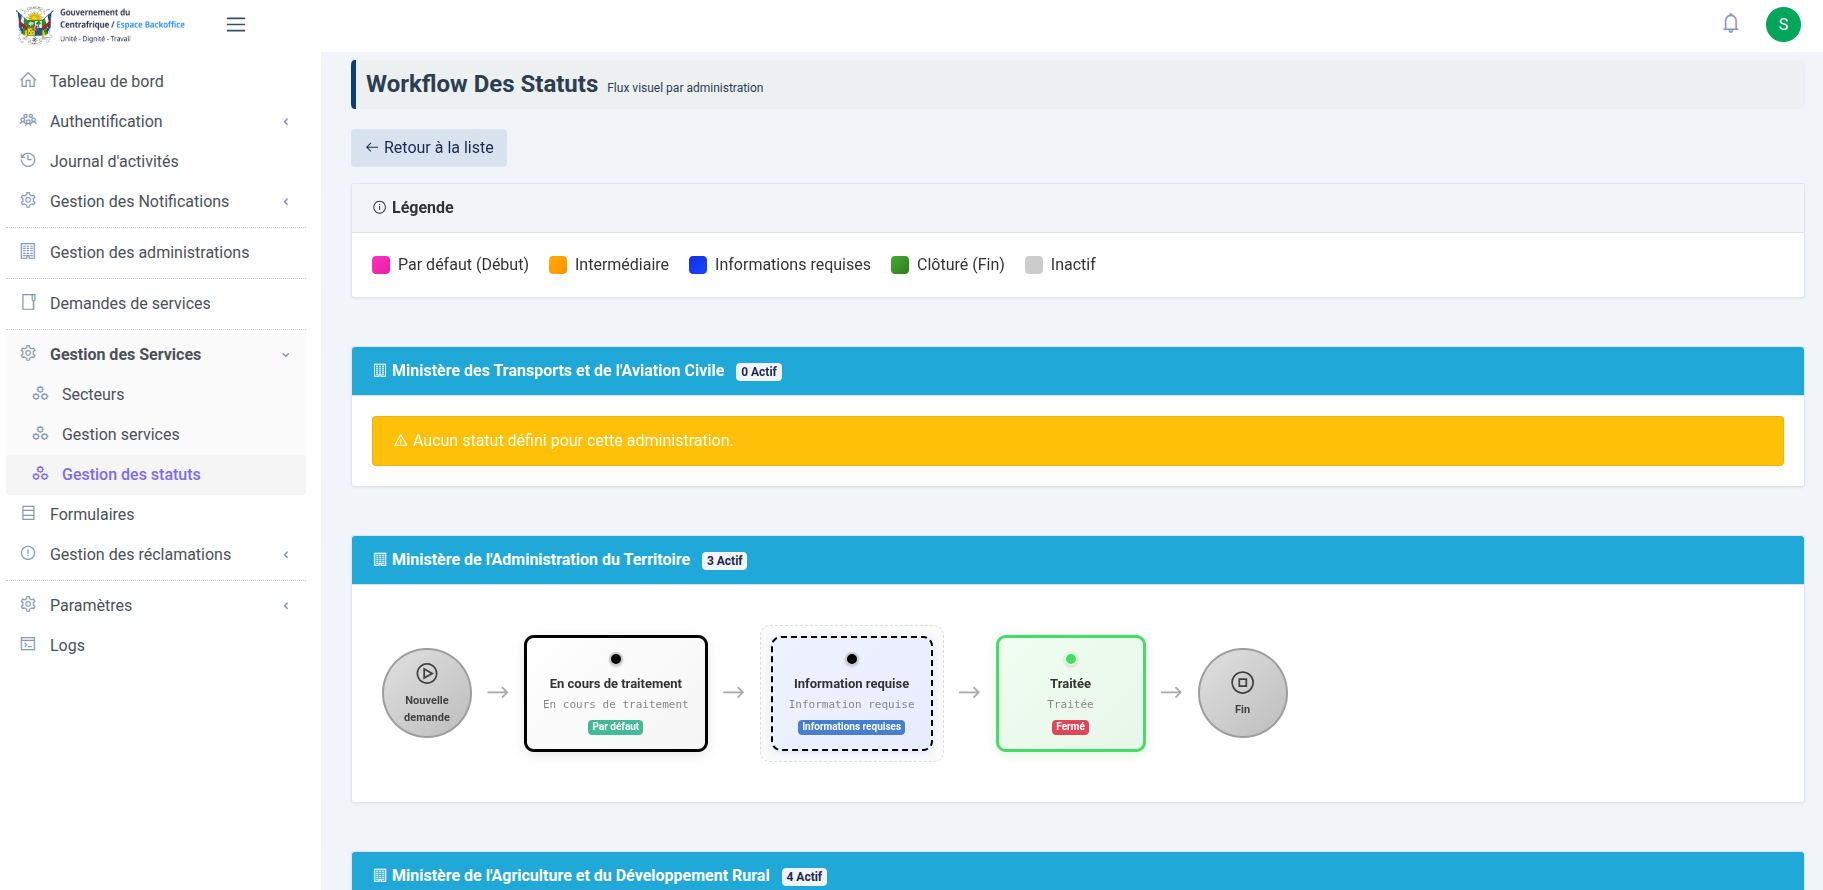
\includegraphics[width=0.95\textwidth]{images/realisation/sprint4/workflow.png}
    }
    \caption{Visualisation du workflow de traitement par administration}
    \label{fig:workflow-traitement}
\end{figure}

% ===================== MODIFIER =====================
La figure~\ref{fig:modifier-etape} présente l’interface qui permet à l’administrateur de modifier une étape existante du workflow. Elle offre la possibilité de mettre à jour les informations liées à une étape de traitement.

\begin{figure}[H]
    \centering
    \fbox{%
        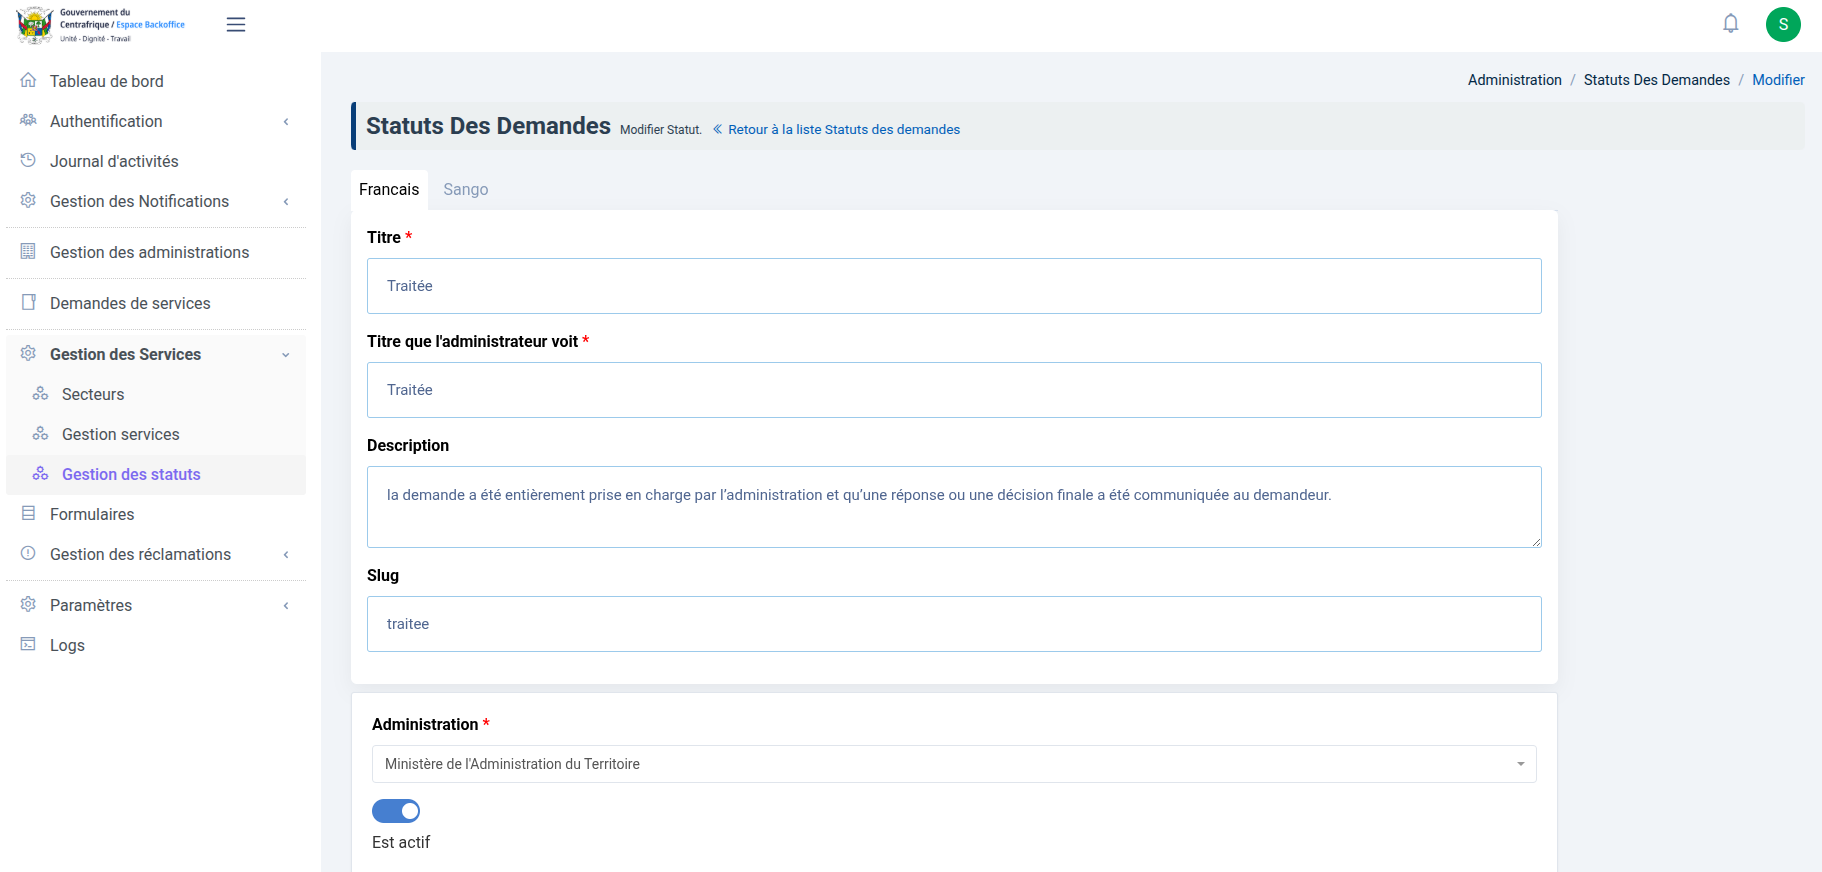
\includegraphics[width=0.95\textwidth]{images/realisation/sprint4/modifier.png}
    }
    \caption{Modification d’une étape}
    \label{fig:modifier-etape}
\end{figure}


% ===================== SUPPRIMER =====================
L'écran illustré en figure ~\ref{fig:suppression-etape} permet à l'administrateur de supprimer une étape du workflow dédié au traitement des réclamations. Un message de confirmation s'affiche au préalable, de manière à prévenir toute suppression involontaire. 

\begin{figure}[H]
    \centering
    \fbox{%
        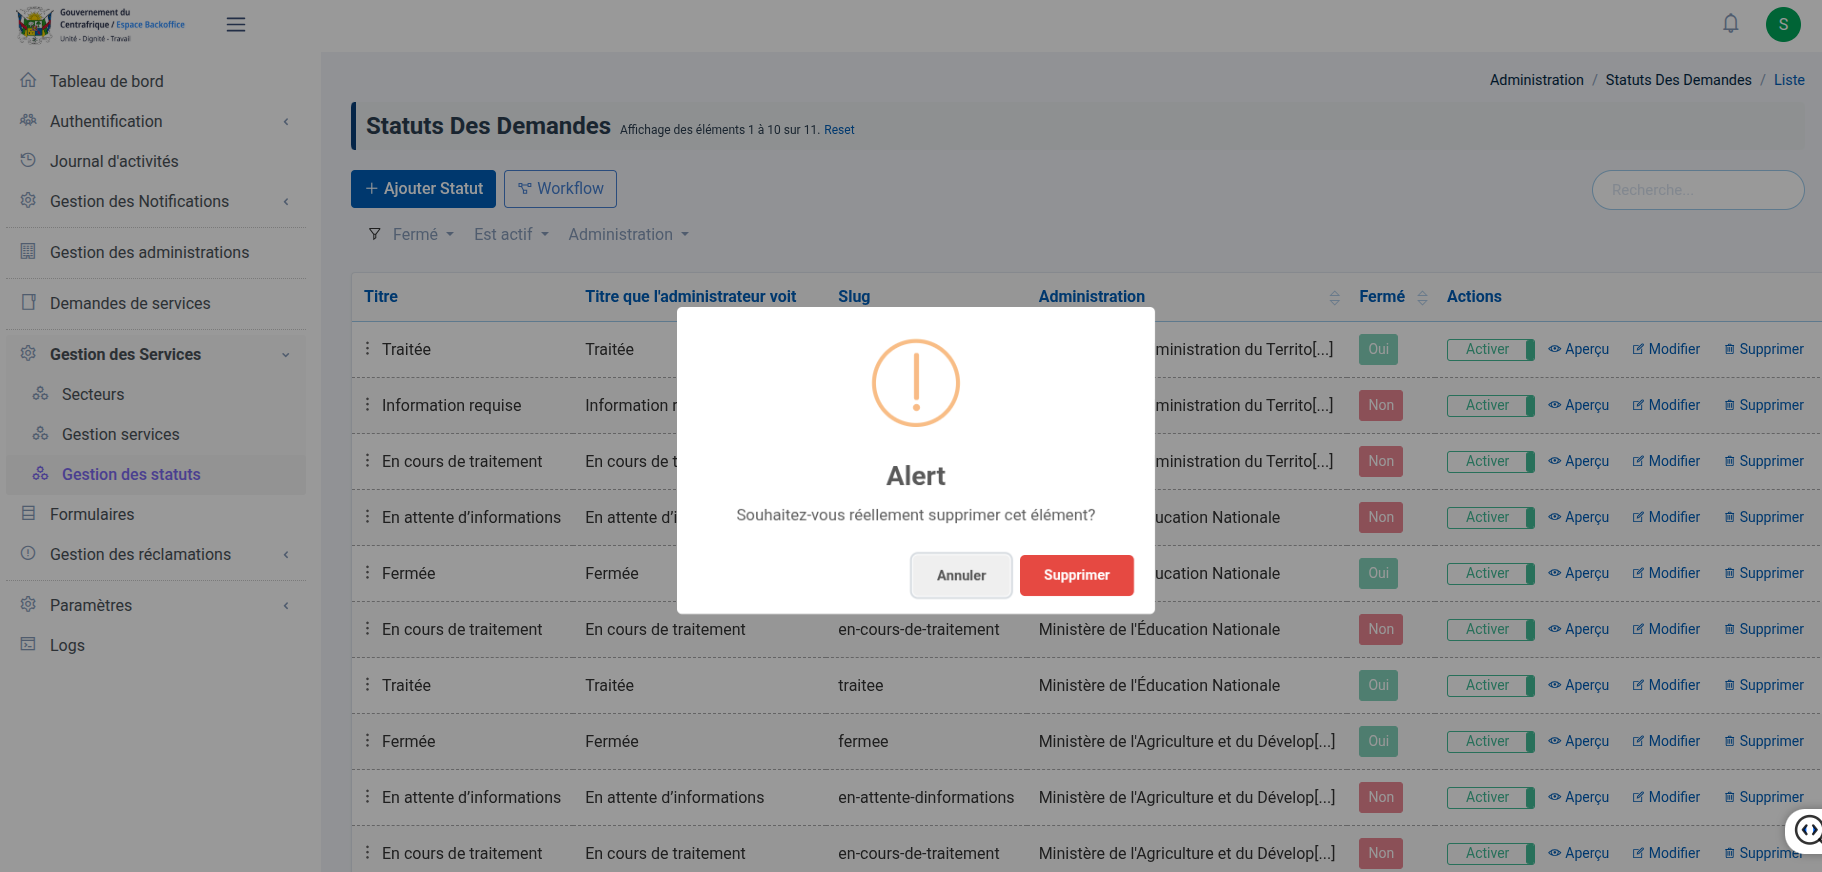
\includegraphics[width=0.95\textwidth]{images/realisation/sprint4/delete.png}
    }
    \caption{Suppression d’une étape}
    \label{fig:suppression-etape}
\end{figure}

\subsection{Réalisation de la supervision de la plateforme}

Le module de supervision donne aux administrateurs une vue d'ensemble de l'activité de la plateforme.

Le tableau de bord de supervision, présenté en figure ~\ref{fig:dashboard-statistiques}, regroupe les statistiques globales relatives aux services et aux réclamations, avec des indicateurs pouvant être répartis selon l'administration concernée ou la période sélectionnée.

\begin{figure}[H]
    \centering
    \fbox{%
        \includegraphics[width=0.95\textwidth]{images/realisation/sprint5/statistique2.png}
    }
    \caption{Tableau de bord des statistiques globales de la plateforme}
    \label{fig:dashboard-statistiques}
\end{figure}

La figure~\ref{fig:journaux-activite} présente l’interface qui permet à l'administrateur de consulter les journaux d'activités de la plateforme et de les filtrer.

\begin{figure}[H]
    \centering
    \fbox{%
        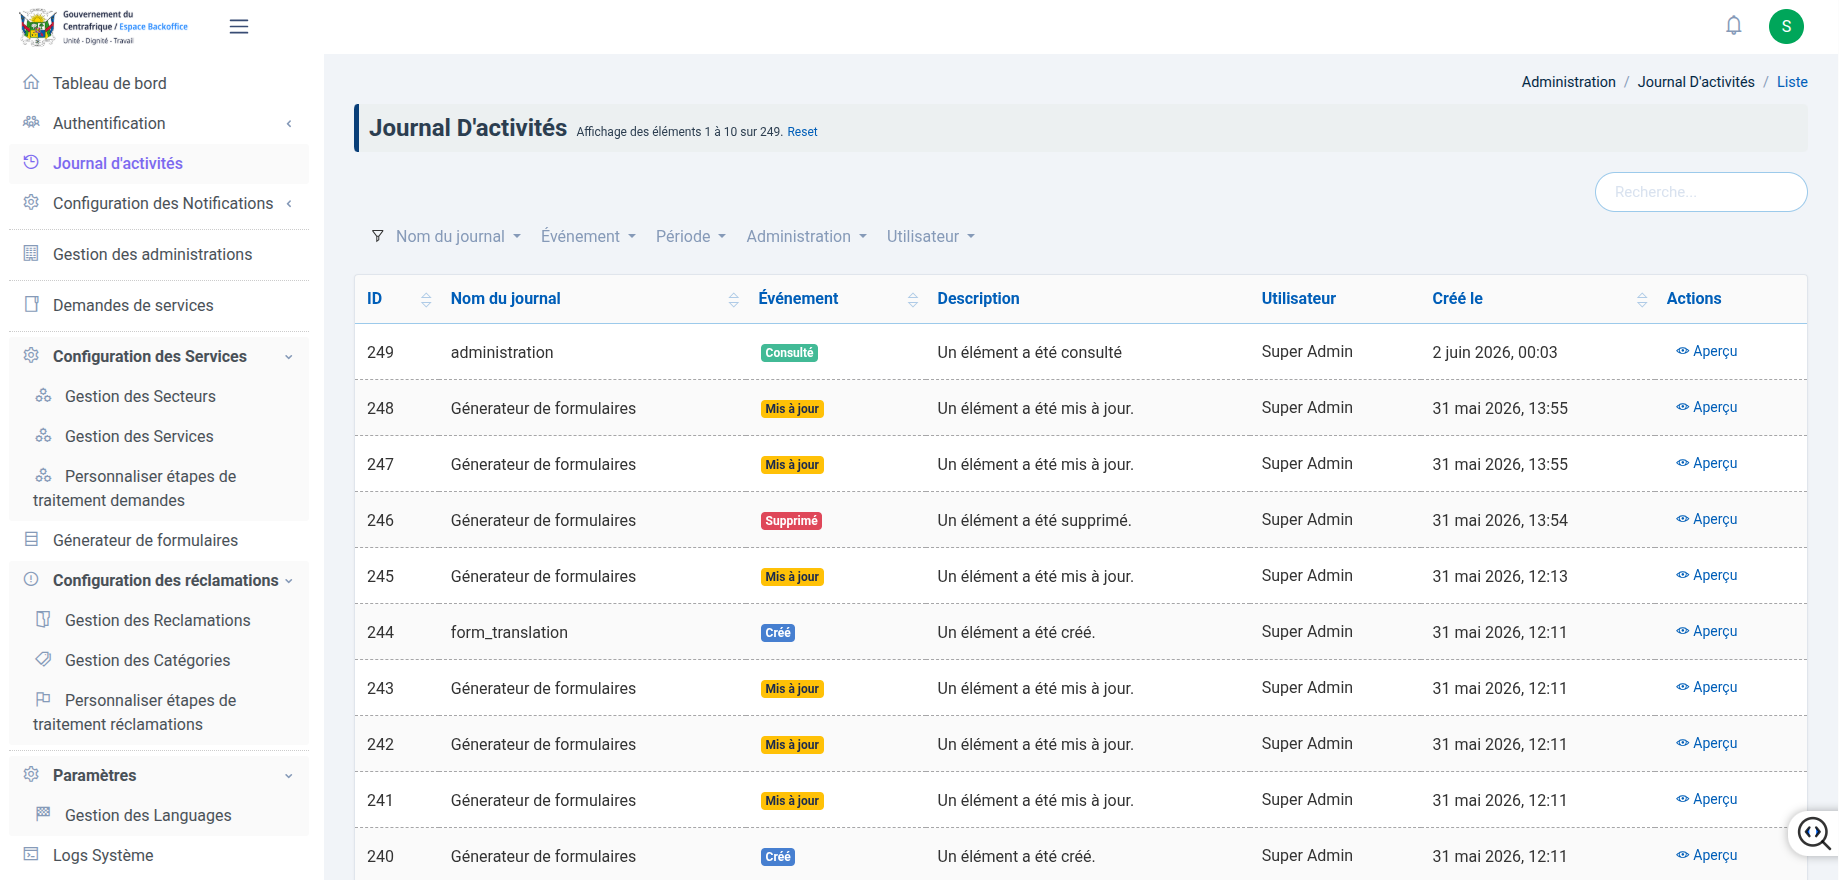
\includegraphics[width=0.95\textwidth]{images/realisation/sprint5/journaux.png}
    }
    \caption{Journaux d’activité}
    \label{fig:journaux-activite}
\end{figure}








Les logs système restituent les événements techniques de la plateforme et aident à détecter les anomalies.


\subsection{Revue du Sprint 4}
 

A l'issue du Sprint 4, l'ensemble des user stories planifiées ont été développées et validées, comme présenté dans le tableau~\ref{tab:revue-sprint4}.

\begin{longtable}{|c|p{9cm}|c|}
\hline
\rowcolor{orange!30}
\textbf{ID} & \textbf{User Story} & \textbf{Statut} \\ \hline
US22 & Gérer les catégories de réclamations & \textcolor{green!60!black}{Terminé} \\ \hline
US23 & Personnaliser les étapes de traitement des réclamations & \textcolor{green!60!black}{Terminé} \\ \hline
US24 & Gérer les réclamations soumises & \textcolor{green!60!black}{Terminé} \\ \hline
US25 & Gérer les modèles de notifications & \textcolor{green!60!black}{Terminé} \\ \hline
US26 & Gérer les notifications & \textcolor{green!60!black}{Terminé} \\ \hline
US27 & Consulter l'historique des notifications & \textcolor{green!60!black}{Terminé} \\ \hline
US28 & Gérer mes réclamations (Internaute) & \textcolor{green!60!black}{Terminé} \\ \hline
US29 & Consulter mes notifications (Client) & \textcolor{green!60!black}{Terminé} \\ \hline
US30 & Consulter les statistiques globales & \textcolor{green!60!black}{Terminé} \\ \hline
US31 & Consulter les journaux d'activités & \textcolor{green!60!black}{Terminé} \\ \hline
US32 & Consulter les logs système & \textcolor{green!60!black}{Terminé} \\ \hline
\caption{Revue du Sprint 4}
\label{tab:revue-sprint4}
\end{longtable}

\section{Sprint 5 : Portail public et assistant conversationnel intelligent}
Le sprint 5 réunit la couche publique de la plateforme et sa composante d'intelligence artificielle. Il met en place la vitrine institutionnelle, qui donne aux internautes un accès public aux informations officielles du gouvernement, et un assistant conversationnel intelligent pour les citoyens. Cet assistant repose sur l'intelligence artificielle générative et une approche \textit{RAG} (\textit{Retrieval-Augmented Generation}, génération augmentée par la recherche) : il répond en langage naturel aux questions des citoyens sur les services, les secteurs, les démarches, les actualités et la FAQ, et réduit la charge pesant sur les canaux de support traditionnels. Le sprint met également en place un canal d'assistance humaine : un citoyen en difficulté laisse ses coordonnées afin d'être recontacté par un administrateur, les demandes étant centralisées et traitées dans le backoffice.


\subsection{Concepts fondamentaux}
Avant de décrire l'assistant, nous rappelons les notions sur lesquelles il repose.

\begin{itemize}
    \item \textbf{Grand modèle de langage (LLM)} : un modèle entraîné à produire du texte en langage naturel. Utilisé seul, il peut « halluciner », c'est-à-dire produire une réponse plausible mais fausse, car il répond à partir de ce qu'il a appris et non à partir des données du portail.
    \item \textbf{Embedding} : la transformation d'un texte en un vecteur de nombres qui en capture le sens. Deux textes proches par le sens donnent des vecteurs proches dans l'espace vectoriel.
    \item \textbf{Base de données vectorielle} : une base qui stocke ces vecteurs et retrouve, pour une requête donnée, les vecteurs les plus proches au sens d'une mesure de similarité (ici la similarité cosinus).
    \item \textbf{RAG (Retrieval-Augmented Generation)} : une approche qui, au lieu de laisser le modèle répondre de mémoire, récupère d'abord les passages pertinents du contenu du portail, puis les fournit au modèle comme contexte. La réponse est ainsi ancrée dans les données réelles, ce qui réduit les hallucinations.
\end{itemize}

\subsection{Backlog du Sprint 5}

Le tableau~\ref{tab:user-stories-sprint5} présente le backlog du cinquième sprint avec l'estimation en jours de chaque tâche. L'ordre des tâches suit une contrainte de dépendance : la vitrine et les pages d'information (notamment les actualités) sont réalisées d'abord, car l'assistant conversationnel est développé ensuite et son indexation (RAG) a besoin de ce contenu pour répondre.

 \renewcommand{\arraystretch}{1.3}

\begin{longtable}{|p{1cm}|p{3cm}|p{7cm}|p{1cm}|p{2cm}|}

\hline
\rowcolor{orange!30}
\textbf{ID} & \textbf{En tant que} & \textbf{User Story} & \textbf{Est/J} & \textbf{Priorité} \\ 
\hline
\endfirsthead

 

US33 & Internaute & 
Je veux consulter les pages d'information (accueil, gouvernement, projets et réalisations, actualités, FAQ, guide, à propos) afin d'accéder aux données officielles du portail & 
2 & Moyenne \\ \hline

US34 & Internaute & 
Je veux contacter l'administrateur afin de poser une question ou signaler un problème & 
1 & Basse \\ \hline

US35 & Internaute & 
Je veux poser des questions à l'assistant conversationnel afin d'obtenir des réponses instantanées sur les services, les secteurs et les démarches (avec saisie vocale, suggestions et possibilité de demander une assistance humaine) & 
14 & Élevée \\ \hline

US36 & Administrateur Système & 
Je veux gérer les demandes d'assistance afin d'accompagner les citoyens & 
2 & Élevée \\ \hline

US37 & Administrateur Système & 
Je veux être notifié par email d'une nouvelle demande d'assistance afin de réagir rapidement & 
1 & Moyenne \\ \hline


\caption{Backlog du Sprint 5}
\label{tab:user-stories-sprint5}

\end{longtable}

 

\subsubsection{Diagramme de cas d'utilisation du Sprint 5}
La figure \ref{fig:cas-utilisation-sprint5} montre le diagramme de cas d'utilisation du sprint 5.

\begin{figure}[H]
    \centering
    \includegraphics[width=11cm,height=10cm]{images/diagrammes/sprint5/v2-cas-utilisation-sprint5.drawio (3).png}
    \caption{Diagramme de cas d'utilisation du Sprint 5}
    \label{fig:cas-utilisation-sprint5}
\end{figure}

\subsubsection{Diagramme de classe -- Sprint 5}
Ce diagramme de classe regroupe les demandes du chatbot et du formulaire de contact.
 La figure \ref{fig:classe-sprint5} montre le diagramme de classe du sprint 5.


\begin{figure}[H]
    \centering
    \includegraphics[width=14cm,height=10cm]{images/diagrammes/sprint5/diag-classe-sprint5.drawio.png}
    \caption{Diagramme de classe du Sprint 5}
    \label{fig:classe-sprint5}
\end{figure}

\subsection{Raffinement et description textuelle du cas d'utilisation << Poser des questions à l’assistant conversationnel >>}

Dans la section suivante, nous utiliserons des descriptions de
scénarios pour décrire le cas « Poser des questions à l’assistant conversationnel ». Ce dernier montre les sous-opérations possibles à faire.

La figure \ref{fig:cas-utilisation-sprint5-raff}, présente le diagramme de cas d'utilisation raffiné du cas d'utilisation « Poser des questions à l’assistant conversationnel ».

\begin{figure}[H]
    \centering
    \includegraphics[width=15cm,height=8cm]{images/diagrammes/sprint5/Copie de v2-cas-utilisation-sprint5.drawio.png}
    \caption{Raffinement du cas d'utilisation « Poser des questions à l’assistant conversationnel »}
    \label{fig:cas-utilisation-sprint5-raff}
\end{figure}


\subsubsection{Descriptions textuelles des cas d'utilisation}
Nous détaillons ci-dessous les deux cas d'utilisation principaux du sprint 5 : l'interaction du citoyen avec l'assistant conversationnel et le traitement des demandes d'assistance par l'administrateur.

 Une description détaillée du cas d'utilisation « Poser une question à l'assistant » est présentée dans le tableau~\ref{tab:desc-poser-question}.

\renewcommand{\arraystretch}{1.3}

\begin{longtable}{|p{4cm}|p{12cm}|}

\hline
\textbf{Champ} & \textbf{Description} \\ \hline
\endfirsthead

 

Nom & Poser une question à l'assistant \\ \hline

Acteur principal & Internaute (citoyen) \\ \hline

Objectif & Obtenir une réponse en langage naturel, fondée sur le contenu du portail. \\ \hline

Pré-condition &
\begin{itemize}
    \item Le contenu du portail est indexé dans la base vectorielle.
\end{itemize}
\\ \hline

Scénario nominal &
\begin{enumerate}
\item L'internaute ouvre l'assistant et saisit (ou dicte) sa question.
\item Le système vectorise la question et recherche les passages pertinents dans l'index Pinecone.
\item Les passages retenus sont transmis au modèle de langage comme contexte.
\item Le système affiche une réponse claire et fidèle au contenu, accompagnée des liens utiles le cas échéant.
\end{enumerate}
\\ \hline

Scénario alternatif &
\begin{itemize}
\item \textbf{Saisie vocale} : au lieu de taper, l'internaute dicte sa question à la voix ; le navigateur transcrit la dictée en texte avant l'envoi.

\item \textbf{Suggestions de questions} : dès l'ouverture, l'internaute peut sélectionner une question prédéfinie pour être guidé au lieu de formuler la sienne.

\item \textbf{Demande d'assistance humaine} : si l'internaute n'arrive pas à obtenir d'aide, il peut demander à être assisté par un administrateur ; le chatbot affiche un court formulaire (nom et téléphone) et enregistre la demande pour un rappel.

\item Si aucun passage pertinent n'est trouvé, l'assistant l'indique sans inventer de réponse.
\end{itemize}
\\ \hline

\caption{Description textuelle - Poser une question à l'assistant}
\label{tab:desc-poser-question}

\end{longtable}

\subsection{Architecture de l'assistant conversationnel}
L'assistant repose sur l'écosystème de modules \textit{AI} de Drupal — \textit{AI Core}, \textit{AI Assistant API}, \textit{AI Chatbot}, \textit{AI Search} et \textit{AI Agents} — complété par deux connecteurs : \textit{AI Provider OpenAI} pour le modèle de langage et la vectorisation, et \textit{AI VDB Provider Pinecone} pour la base de données vectorielle \textit{Pinecone}. Le fournisseur Gemini a également été évalué (voir la section sur le choix du fournisseur LLM). Le tableau \ref{tab:modules-ai} décrit le rôle de chaque module.

\renewcommand{\arraystretch}{1.3}

\begin{longtable}{|p{4.5cm}|p{10.5cm}|}

\hline
\rowcolor{orange!30}
\textbf{Module} & \textbf{Rôle} \\ \hline
\endfirsthead

\hline
\rowcolor{orange!30}
\textbf{Module} & \textbf{Rôle} \\ \hline
\endhead


AI Core & 
Couche de base de l'écosystème ; fournit l'abstraction commune aux fournisseurs d'IA et l'API utilisée par les autres modules. 
\\ \hline

AI Provider OpenAI & 
Connecteur vers OpenAI ; permet d'appeler le modèle \texttt{gpt-4o} pour la génération des réponses et le modèle \texttt{text-embedding-3-large} pour la vectorisation (\textit{embeddings}). 
\\ \hline

AI VDB Provider Pinecone & 
Connecteur vers la base de données vectorielle Pinecone ; enregistre et interroge les vecteurs du contenu. 
\\ \hline

AI Search & 
Met en œuvre la recherche sémantique (RAG) ; indexe le contenu du portail et récupère les passages les plus pertinents via Search API. 
\\ \hline

AI Assistant API & 
Définit l'assistant conversationnel : ses instructions, son comportement et ses sources de contexte. 
\\ \hline

AI Chatbot & 
Fournit l'interface de conversation (\textit{widget}) intégrée au portail. 
\\ \hline


\caption{Modules de l'écosystème AI de Drupal utilisés}
\label{tab:modules-ai}

\end{longtable}

\subsection{Pipeline RAG}
\noindent Le fonctionnement de l'assistant suit deux phases. La première, hors ligne, indexe le contenu : chaque contenu du portail est découpé en passages (\textit{chunking}), converti en \textit{embedding} par le modèle de vectorisation, puis enregistré dans l'index Pinecone. La seconde, en ligne, traite la question : la question est vectorisée, comparée aux vecteurs de l'index par similarité, et les passages les plus proches sont fournis au modèle de langage comme contexte pour produire la réponse. La figure \ref{fig:schema-rag} illustre ces deux phases.

\begin{figure}[H]
    \centering
    \includegraphics[width=\textwidth]{images/diagrammes/sprint5/schema-rag.drawio.png}
    \caption{Pipeline RAG de l'assistant conversationnel}
    \label{fig:schema-rag}
\end{figure}

\subsection{Base de données vectorielle}
\noindent La base vectorielle est le socle de la phase de recherche du RAG. Le projet s'appuie sur \textit{Pinecone}, une base de données vectorielle gérée dans le cloud, à travers un index dédié (collection \texttt{trainning}, métrique cosinus, vecteurs de 3072 dimensions).

\noindent Chaque contenu du portail est découpé en passages (taille de passage de 2000 caractères, chevauchement de 100), puis converti en \textit{embedding} à l'aide du modèle \texttt{text-embedding-3-large} d'OpenAI. Ces vecteurs sont enregistrés dans l'index Pinecone. Lorsqu'une question est posée, elle est à son tour vectorisée puis comparée aux vecteurs de l'index par \textbf{similarité sémantique}, afin d'extraire les passages les plus proches.

\noindent Le comportement de la recherche est paramétrable :
\begin{itemize}
    \item \textbf{Seuil de similarité} : score minimal qu'un passage doit atteindre pour être retenu ;
    \item \textbf{Nombre de résultats} : nombre maximal de passages fournis au modèle comme contexte ;
    \item \textbf{Mode de restitution} : passages bruts (\textit{chunks}) ou contenus rendus.
\end{itemize}

\subsection{Choix du fournisseur LLM et configuration des clés API}
\noindent Le module \textit{AI} de Drupal s'interface avec le modèle de langage via un fournisseur configurable. La clé d'accès (\textit{clé API}) est enregistrée de manière sécurisée dans le gestionnaire de clés (\textit{Key}) de Drupal plutôt qu'en clair dans le code. Deux fournisseurs ont été testés avant d'arrêter le choix définitif. La vectorisation et la génération sont assurées par deux modèles distincts d'OpenAI : \texttt{text-embedding-3-large} pour les embeddings et \texttt{gpt-4o} pour la génération des réponses.

\begin{itemize}
    \item \textbf{Gemini (Google)}, modèles \texttt{gemini-embedding-2-preview}
    (embeddings) et \texttt{gemini-2.0-flash} (génération) : intégrés et
    fonctionnels, mais affectés par une connectivité réseau instable depuis
    l'environnement de développement (résolution DNS lente vers les services
    Google), entraînant des délais d'attente et des réponses intermittentes.

    \item \textbf{OpenAI}, modèles \texttt{text-embedding-3-large} (embeddings) et \texttt{gpt-4o} (génération) : retenu. Il offre un bon compromis entre coût, rapidité et qualité de restitution en français.
\end{itemize}

\noindent Le tableau \ref{tab:comparaison-llm} synthétise cette comparaison.

\begin{table}[H]
\centering
\begin{tabular}{|p{3cm}|p{3.5cm}|p{2.5cm}|p{3cm}|} \hline
\rowcolor{orange!30}
\textbf{Fournisseur} & \textbf{Connectivité} & \textbf{Coût} & \textbf{Décision} \\ \hline
Gemini & Instable (DNS) & Faible & Écarté \\ \hline
OpenAI & Fiable & Maîtrisé & \textbf{Retenu} \\ \hline
\end{tabular}
\caption{Comparaison des fournisseurs LLM évalués -- Sprint 5}
\label{tab:comparaison-llm}
\end{table}

\subsection{Réalisation du Sprint 5}

\noindent \textbf{Vitrine institutionnelle :}

La figure~\ref{fig:accueil-vitrine} présente la vitrine. Cette  vitrine donne aux internautes un accès public aux informations officielles du portail à travers un ensemble de pages : accueil, gouvernement, projets et réalisations, actualités, FAQ, guide d'utilisation et à propos.

\begin{figure}[H]
    \centering
    \fbox{%
        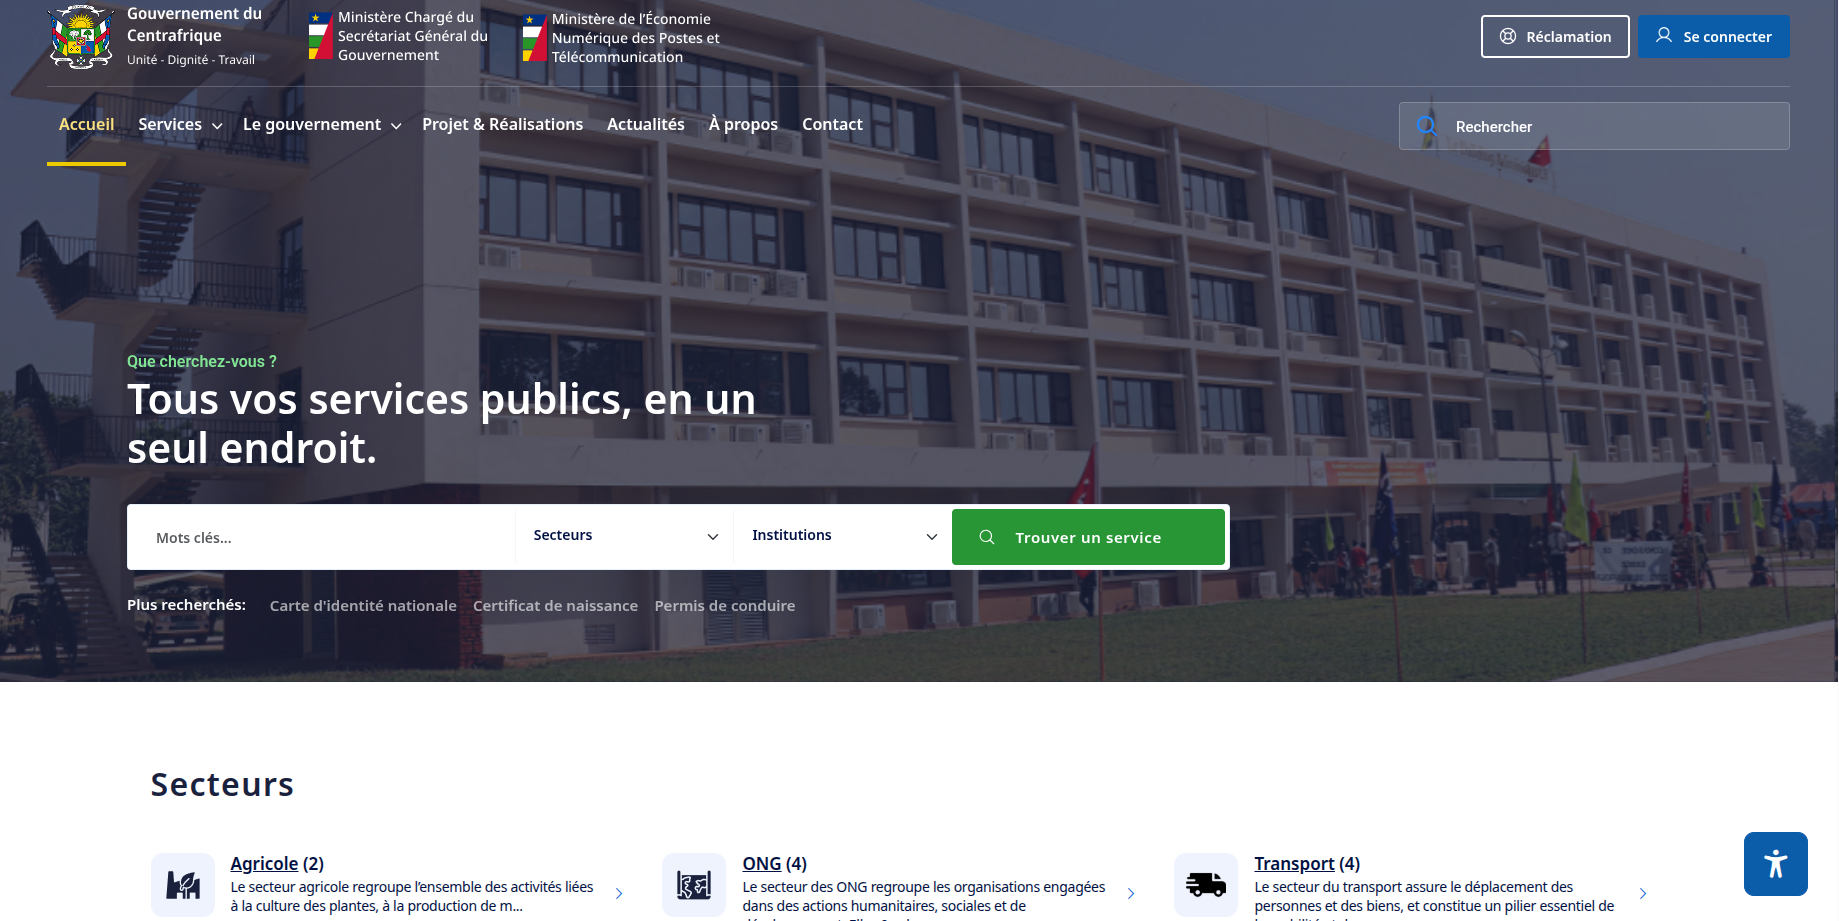
\includegraphics[width=0.95\textwidth]{images/realisation/sprint5/accueil.png}
    }
    \caption{Page d’accueil de la vitrine institutionnelle}
    \label{fig:accueil-vitrine}
\end{figure}


La figure~\ref{fig:projets-realisations-vitrine} présente la page « projets et réalisations »  qui présente les initiatives officielles du gouvernement.

\begin{figure}[H]
    \centering
    \fbox{%
        
\includegraphics[width=0.95\textwidth]{images/realisation/sprint5/projet-realisation.png}
    }
    \caption{Page « Projets et réalisations » de la vitrine institutionnelle}
    \label{fig:projets-realisations-vitrine}
\end{figure}






\noindent \textbf{Assistant conversationnel :}

La figure~\ref{fig:real-chatbot} présente l'assistant intégré au portail : il offre une saisie vocale (dictée via le navigateur) et des suggestions de questions qui guident l'internaute dès l'ouverture de la conversation.

\begin{figure}[H]
    \centering
    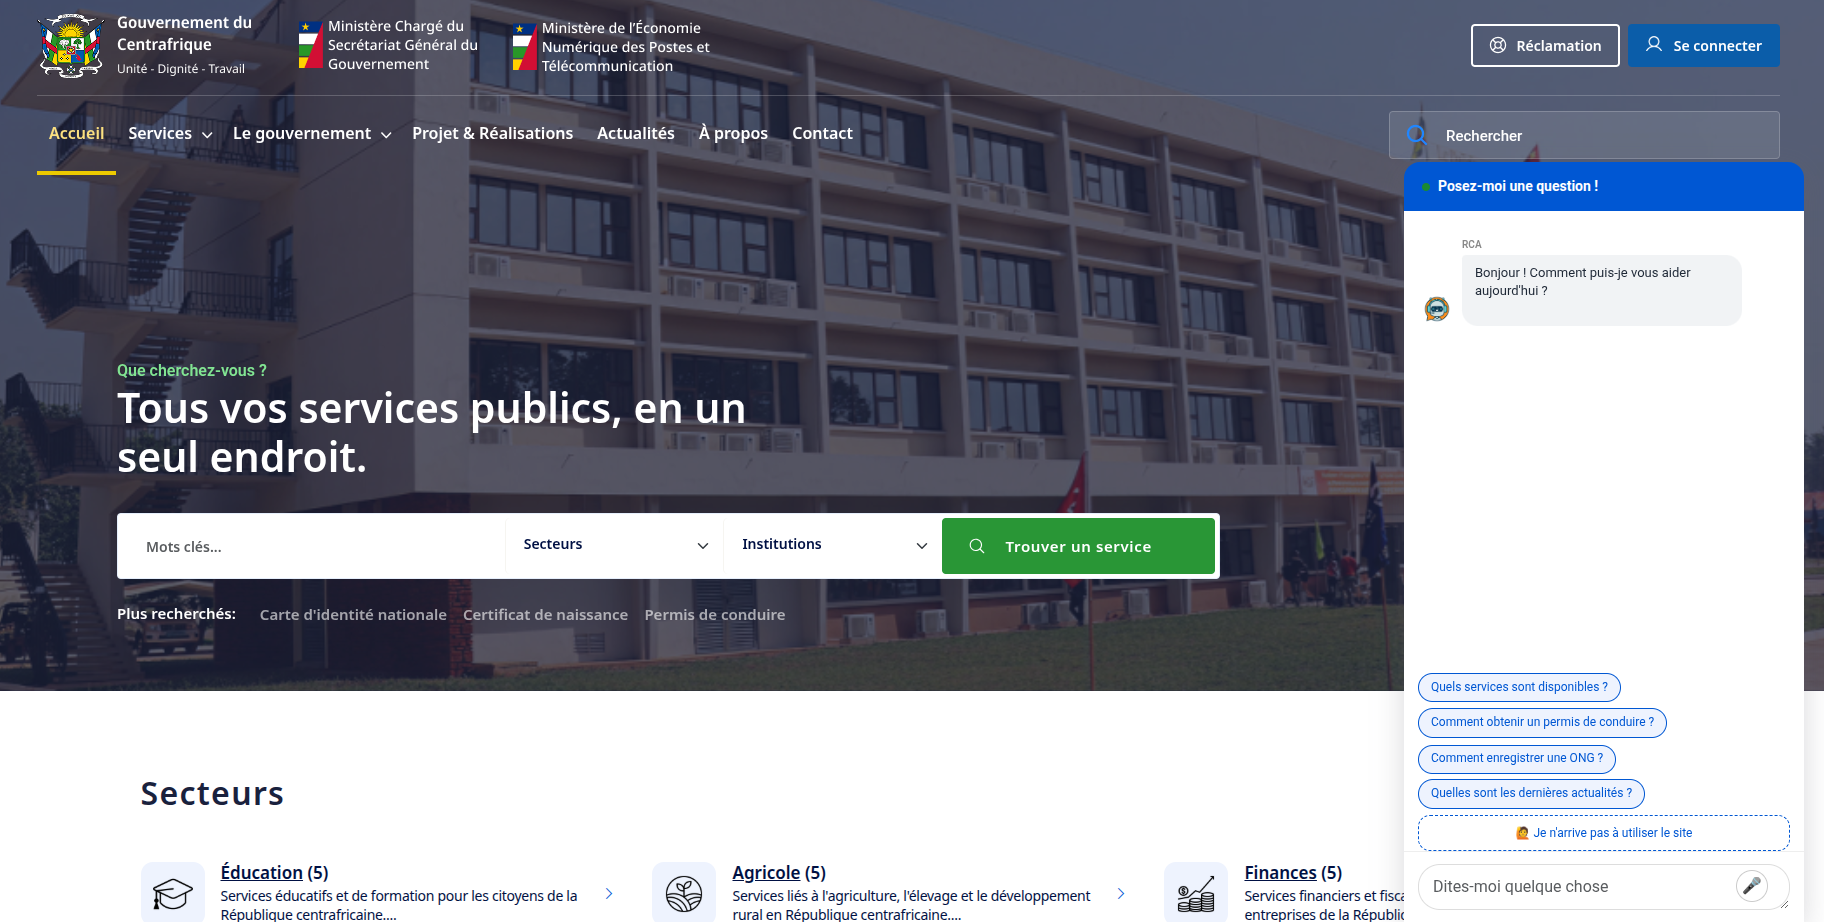
\includegraphics[width=0.95\textwidth]{images/realisation/sprint6/Capture d’écran du 2026-06-14 21-39-48.png}
    \caption{Assistant conversationnel sur le portail}
    \label{fig:real-chatbot}
\end{figure}

La figure~\ref{fig:real-assistance-form} présente une réponse du chatbot fondée sur le contenu indéxe dans la base vectorielle.

\begin{figure}[H]
    \centering
    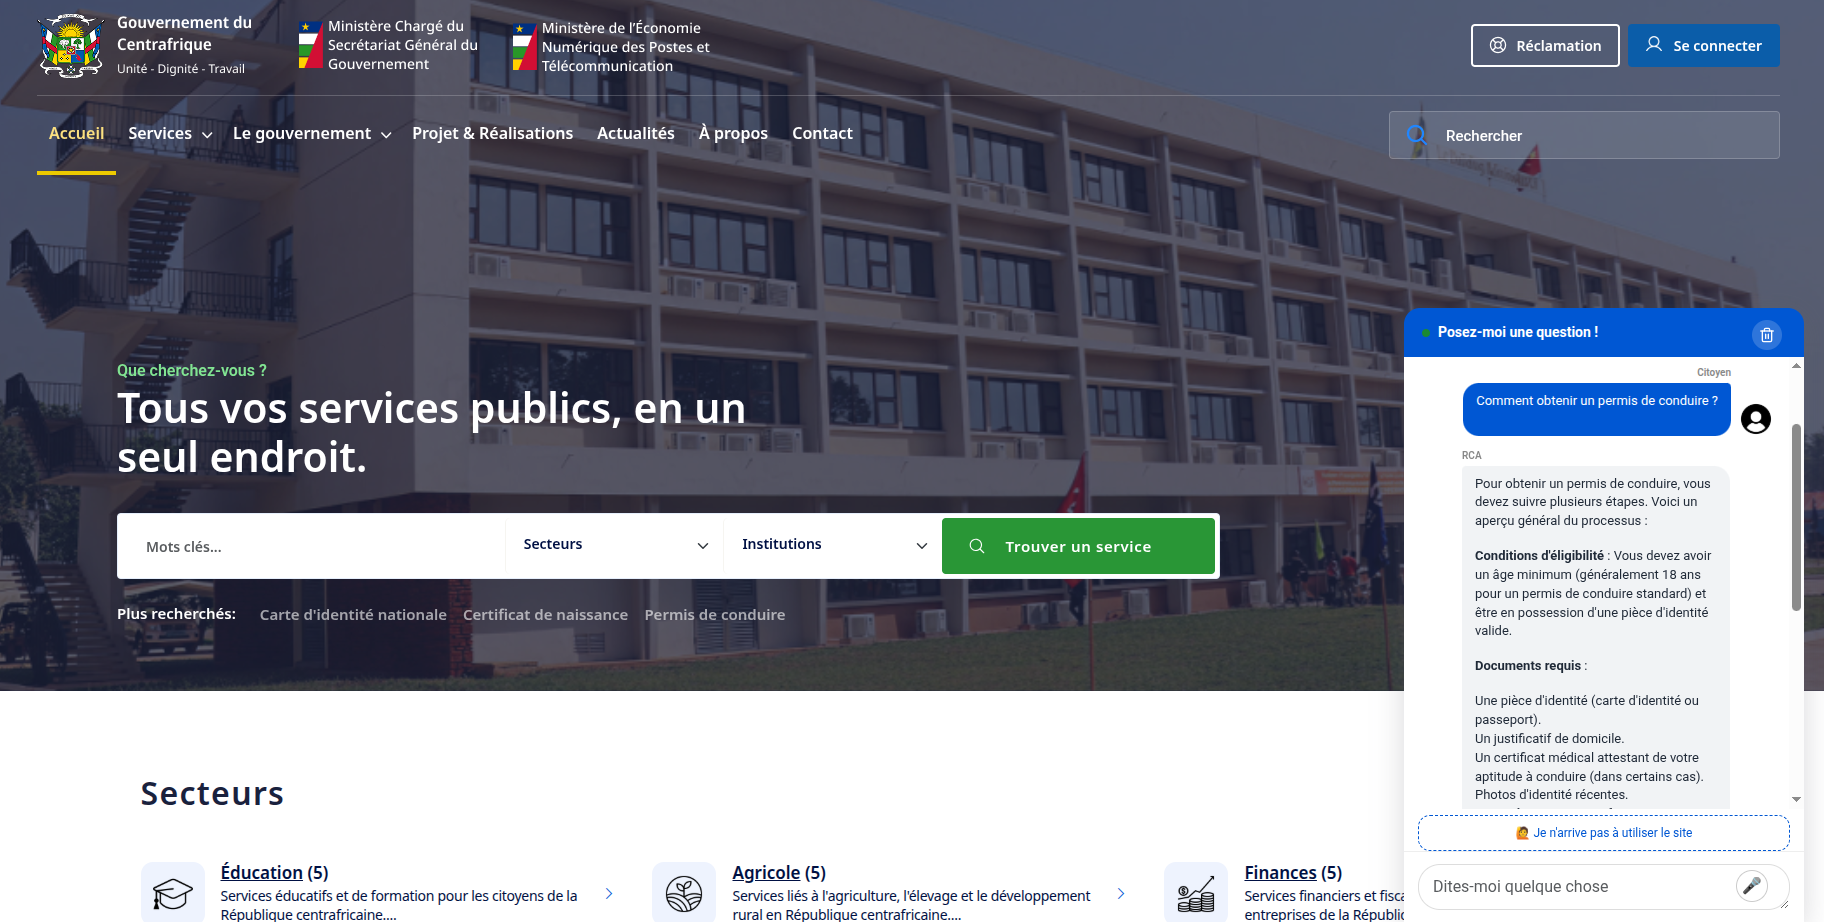
\includegraphics[width=14cm,height=8cm]{images/realisation/sprint6/Capture d’écran du 2026-06-14 21-40-18.png}
    \caption{Demande d'assistance depuis le chatbot}
    \label{fig:real-assistance-form}
\end{figure}

\noindent \textbf{Demande d'assistance depuis le chatbot :}

Lorsqu'un internaute signale une difficulté, l'assistant affiche un court formulaire (nom et téléphone) puis confirme la prise en compte de la demande, comme illustré dans la figure~\ref{fig:real-backoffice-assistance} .


\begin{figure}[H]
    \centering
    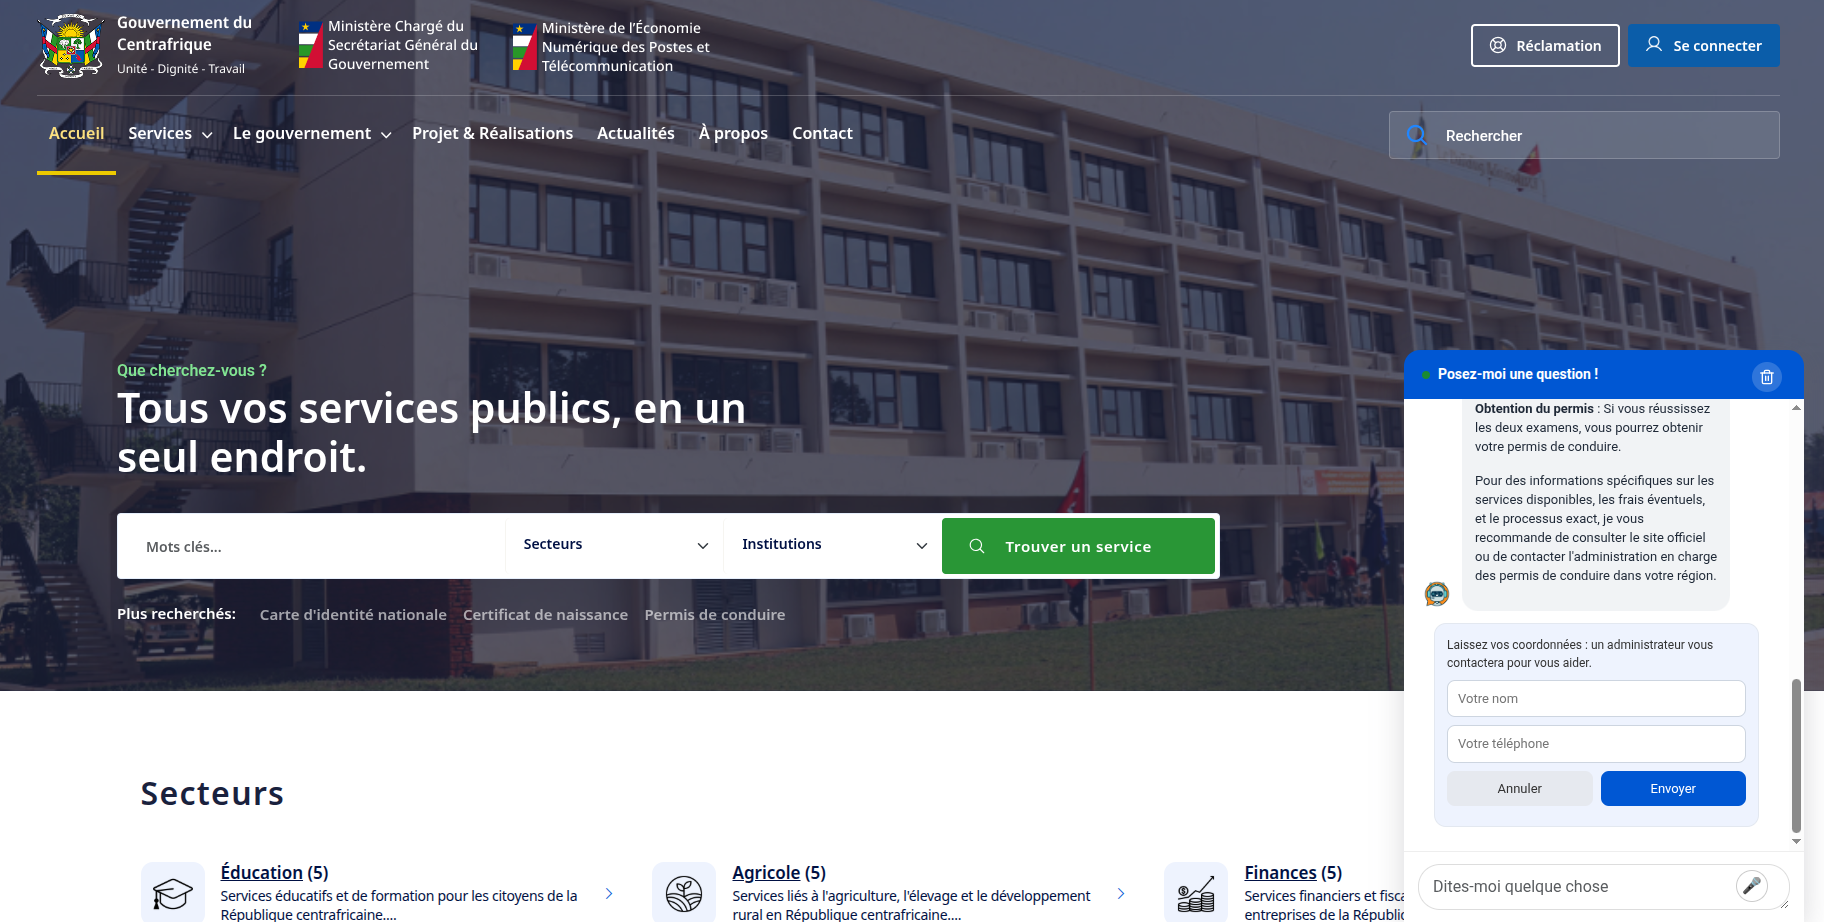
\includegraphics[width=14cm,height=8cm]{images/realisation/sprint6/Capture d’écran du 2026-06-14 21-40-25.png}
    \caption{Gestion des demandes d'assistance dans le backoffice}
    \label{fig:real-backoffice-assistance}
\end{figure}

\noindent \textbf{Gestion des demandes dans le backoffice :}

\noindent Les demandes, qu’elles proviennent du chatbot ou du formulaire de contact, sont centralisées au niveau du backoffice, où l’administrateur peut les consulter, les filtrer selon leur statut et faire évoluer leur traitement. Ce processus est illustré par la figure~\ref{fig:real-gestion-assistance}.
 
\begin{figure}[H]
    \centering
    \fbox{%
        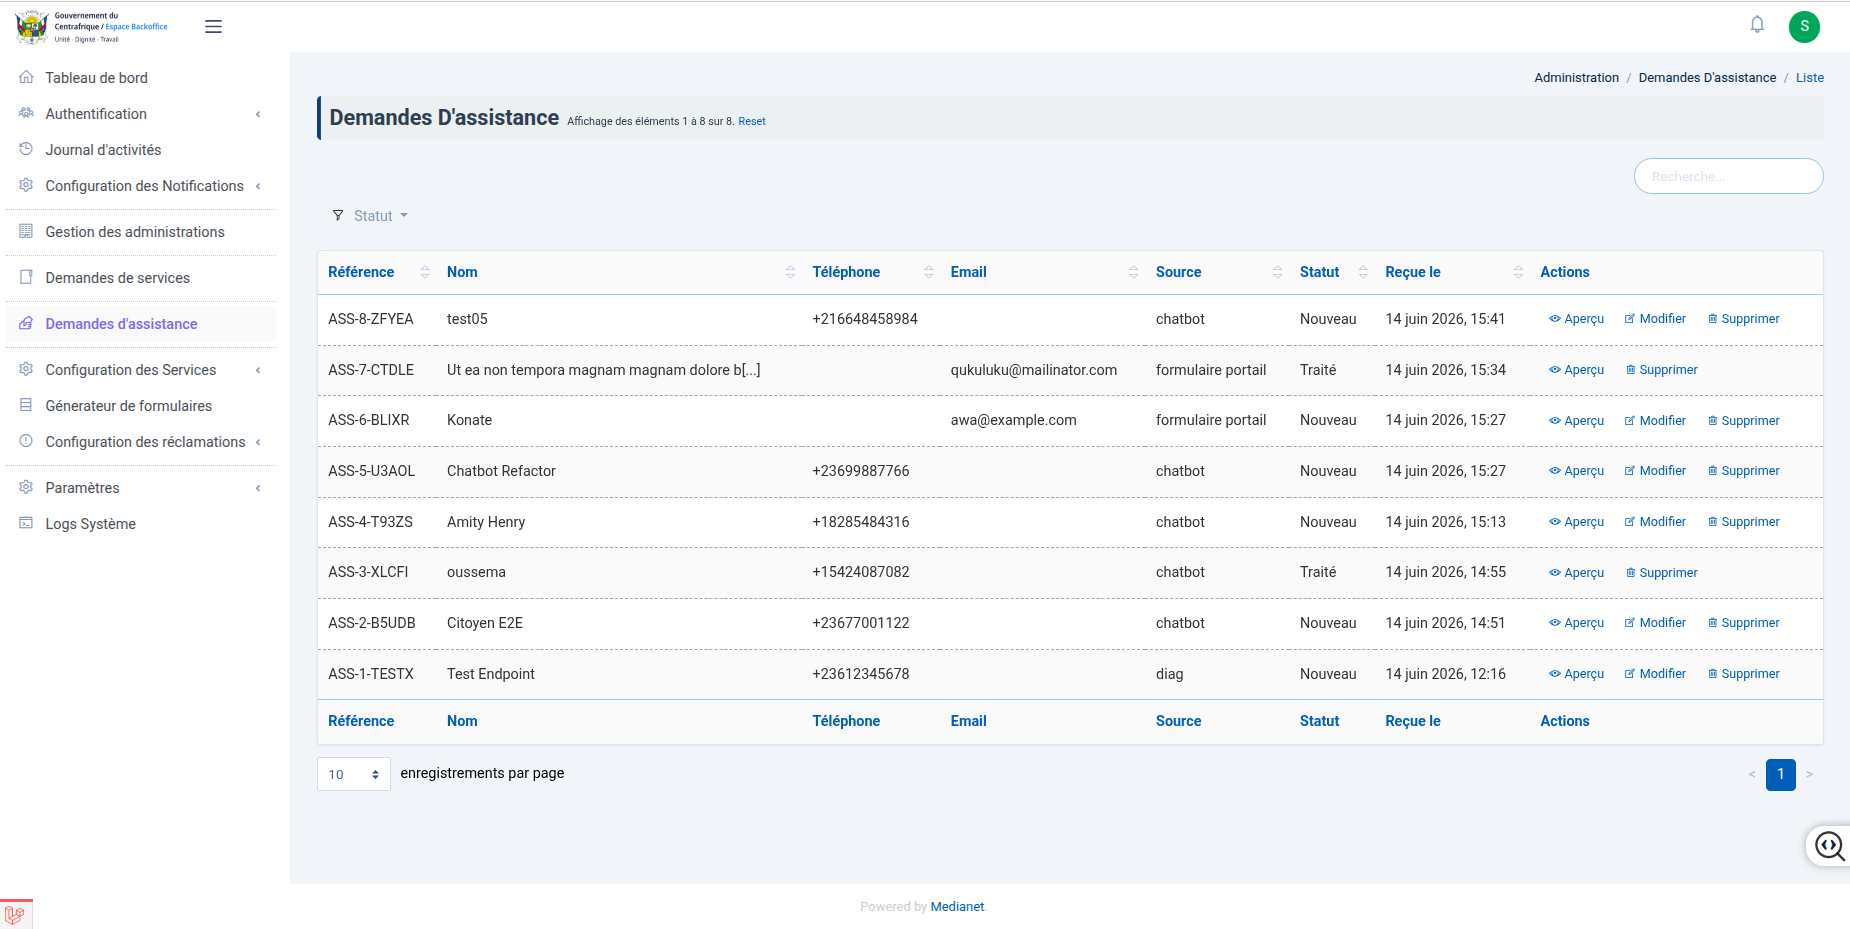
\includegraphics[width=0.95\textwidth]{images/realisation/sprint6/Capture d’écran du 2026-06-14 21-45-07.png}
    }
    \caption{Page de gestion des demandes d’assistance}
   \label{fig:real-gestion-assistance}
\end{figure}





\subsection{Limites et perspectives}
\noindent L'assistant est fonctionnel et ancré dans le contenu du portail, mais plusieurs limites restent à lever.

\begin{itemize}
    \item \textbf{Renforcer la souveraineté des données :} envisager une migration vers une infrastructure entièrement auto-hébergée reposant sur une architecture découplée (par exemple Milvus ou Qdrant pour la base vectorielle, un modèle d'embedding open source et un LLM local tel que Llama ou Mistral). Cette évolution permettrait de traiter des données sensibles, notamment celles des citoyens, tout en garantissant une meilleure maîtrise des informations.

    \item \textbf{Mettre en place un protocole d'évaluation :} élaborer un jeu de questions-réponses de référence afin d'évaluer objectivement les performances du système, notamment en termes de précision et de taux d'hallucination. Des tests de charge réalisés avec des outils comme JMeter ou k6 permettraient également de vérifier la robustesse de la solution.

    \item \textbf{Étendre et automatiser les sources de connaissances :} enrichir progressivement la base documentaire en intégrant de nouvelles sources officielles et automatiser leur collecte ainsi que leur mise à jour afin de garantir des informations fiables et constamment actualisées.
\end{itemize}

\noindent En perspective, l'activation du function calling, un réglage plus fin de l'indexation des actualités et une mise en cache des réponses fréquentes amélioreraient la fiabilité et la rapidité de l'assistant.

\subsection{Revue du Sprint 5}

Le tableau ~\ref{tab:revue-sprint5} récapitule les user stories prévues pour ce sprint, toutes achevées et validées au terme du Sprint 5.

\begin{longtable}{|c|p{9cm}|c|}
\hline
\rowcolor{orange!30}
\textbf{ID} & \textbf{User Story} & \textbf{Statut} \\ \hline
US33 & Consulter les pages d'information & \textcolor{green!60!black}{Terminé} \\ \hline
US34 & Contacter l'administrateur & \textcolor{green!60!black}{Terminé} \\ \hline
US35 & Poser une question à l'assistant conversationnel (voix, suggestions et demande d'assistance incluses) & \textcolor{green!60!black}{Terminé} \\ \hline
US36 & Gérer les demandes d'assistance & \textcolor{green!60!black}{Terminé} \\ \hline
US37 & Être notifié par email d'une nouvelle demande & \textcolor{green!60!black}{Terminé} \\ \hline
\caption{Revue du Sprint 5}
\label{tab:revue-sprint5}
\end{longtable}

\section{Conclusion}

Répartie sur deux sprints, la release 2 a fait l'objet de ce chapitre. D'un côté, le Sprint 4 a été consacré à la mise en place de la gestion des réclamations, du système de notifications et des outils dédiés à la supervision. De l'autre, le Sprint 5 a abouti au déploiement du portail public, comprenant une vitrine institutionnelle ainsi qu'un assistant conversationnel s'appuyant sur une approche RAG, épaulé par un canal d'assistance assuré par des opérateurs humains.
